\documentclass[a4paper]{article}

\usepackage{url}
\usepackage{graphicx}	% For figure environment
\usepackage{epstopdf}
\usepackage[center]{subfigure}
\usepackage{amssymb}	% For mathematical figures like \mathbb{R}
\usepackage{amsmath}
\usepackage{framed}
\usepackage{tikz}
\usetikzlibrary{mindmap,trees}
\usepackage{pdflscape}
\usepackage[a4paper]{geometry}


\title{Advanced Systems Lab - Milestone I} 
\author{Lukas Elmer, Matthias Ganz} 
\date{\today} 


\begin{document}

\maketitle


\begin{abstract}

This document, describes the message queuing system which was build. Architecture and design choices are shown and explained. Further test scenarios and test loads are defined. Resulting test output is described and analysed.

\end{abstract}

%% %%%%%%%%%%%%%%%%%%%%%%%%%%%%%%%%%%%%%%%%%%%%%%
\section{Messaging System}
In this section the system under test (also named as middle ware component) is described.


%% ----------------------------------------------
\subsection{Overview}

Figure \ref{fig:system-overview} shows a generic setup of the messaging system. Multiple middle ware components are connected to a single database and severs a couple of clients. Application state is persisted on the database, therefore a middle ware component can be considered as stateless.

% ------------------------------------------------
% Figure - system overview

\begin{figure}
  \begin{center}
    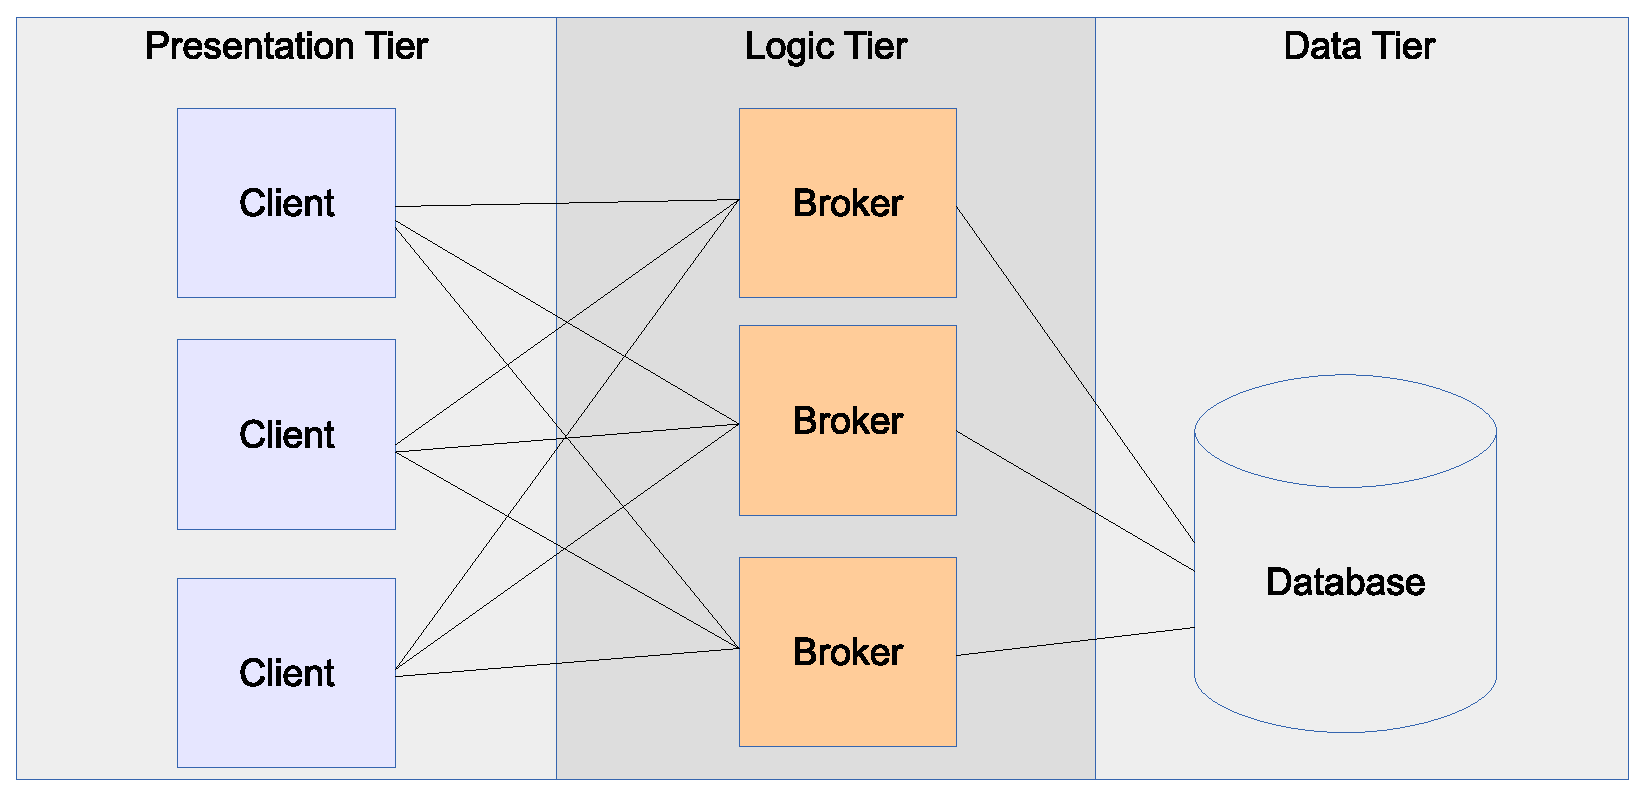
\includegraphics[scale=0.4]{../drawings/system-overview.eps}
  \end{center}
  \caption{System Overview}
  \label{fig:system-overview}
\end{figure}

Figure \ref{fig:middleware-threading} shows important software components of a single middle ware. A nonblocking network interface (NIO) handles communication to the clients. Received data is put to a single thread safe request queue.

A configurable number of workers are constantly reading from the request queue. As soon as a worker gets a piece of work (request raw data) it then performs the following tasks:
\begin{itemize}
\item decoding: The raw request is parsed and converted into a request java object
\item process: The request is processes. The database is accesses and a response object is created
\item encode: The response object is serialized and placed into the response queue of the network interface.
\end{itemize}

% ------------------------------------------------
% Figure - threading

\begin{figure}
	\begin{center}
    \includegraphics[scale=0.4]{../drawings/broker-threading.eps}
  \end{center}
  \caption{Middleware's main Components}
  \label{fig:middleware-threading}
\end{figure}

%% ----------------------------------------------
\section{Design Decisions}
In this section a selection of the more important design decisions is presented. It is described why these choices were made and how they affect the behaviour of the system.

\subsection{Blocking vs. Nonblocking Network IO}
Java basically allows two ways how to handle tcp/ip connections. There is the more straight forward way with blocking io and there is another api which allows nonblocking operation on sockets.

The implementation of the middle ware features a single threaded networking software layer which implements the reactor pattern by using a \textit{java.nio.channels.Selector}. The basic idea is to let the Selector keep track of connections. By a connection based configuration we let the Selector know in which events we are interested in.

\paragraph{Advantages}
By using nonblocking io over the blocking method, we avoid that the number of threads in the system need to be scaled to the number of clients to simultaneously serve. It is assumed that system scales better in terms concurrent connections thant the blocking method for the simple fact that thread switches takes time and memory.

\subsection{Database Connection Pooling}
Establishing a jdbc database connection takes time. A Connection Pool keeps a list of database connections which are permanently opened. As soon as a connection is needed by a worker, it simply queries the pool for one.

The pool needs to be accessed in an exclusive fashion. However the cost to avoid concurrent pool access should be way lower than creating a database connection each time one is needed.

A nice effect of having a permanent database connection is that it allows the use of PreparedStatement. Sql statements which can be precompiled on the database system.

\paragraph{Another option}
Having a connection pool could have been avoided if every client was assigned a dedicated database connection. There would have been no need to synchronize worker threads to retrieve a connection. This however decreases the number of tuning parameter. Database connection would not have been optimally used. Connections would have been idling for each time consuming operation a worker performs.

\subsection{Buffer Pooling}
\label{sub:buffer-pooling}
Serializing and deserializing messages which are up to 2kb long requires a buffer of at least the same size. In order to avoid excessive garbage collection it was decided to implement a pool containing message buffers.

Pooled buffers are obtained from the networking interface before receiving a message. After processing the message and right before we lose the reference to the buffer it is put back to the pool for later use.

Having this pool should significantly increase the period between garbage collection.

\subsection{Message Transmission}
Messages are passed on the initiative of a client (There is no way for the messaging system to push information to a specific client). A clients issues a requests and expects a response within a certain time. Each requests generates a response. In case of an error an error response is replied by the middle ware.

A message consists of a 4 byte length field and a variable length field containing the payload.

To send a messages (requests and responses) the first 4 bytes indicate the binary length of the message. After that the request (or response) is serialized.

\subsection{Message Serialisation}

The first approach to serialize messages was using the java's built in stream based serialisation infrastructure. This however did not work well together with \ref{sub:buffer-pooling}. Default java serialisation won't let us plug in our buffer pool. Furhter the decision to implement the networking interface with java nonblocking io however forced us to use java's \textit{ByteBuffer} class to handle binary data.

Theses issues brought us to the decision to implement custom serialisation and deserialisation supporting pooled ByteBuffers.

\subsection{Load Shedding}
With the current design requests are queued in a single request queue. If workers are slow requests begin to queue up. If the queue is full adding another request fails. The request from the client is silently dropped.


\section{Performance Relevant Features}

\subsection{Overview}

During a brainstorming session, a broad spectrum of performance relevant features were extracted, see figure~\ref{fig:features_mindmap}. Then, the primary features (PF, orange) and the secondary features (SF, green) were chosen according to the group membmers domain specific knowledge and presumptions.
% Later: They were then validated during discussions with other groups and the teachin assistant.


%\begin{landscape}

%\tikzset{concept/.append style={fill={none}}}
\tikzset{concept/.append style={circle}}
\tikzset{level 1 concept/.append style={font=\sf, level distance = 44mm}}
\tikzset{level 2 concept/.append style={font=\sf, level distance = 22mm}}
\tikzset{level 3 concept/.append style={font=\sf, level distance = 22mm}}
\tikzset{every node/.append style={scale=0.8}}
    
\begin{figure}
\center
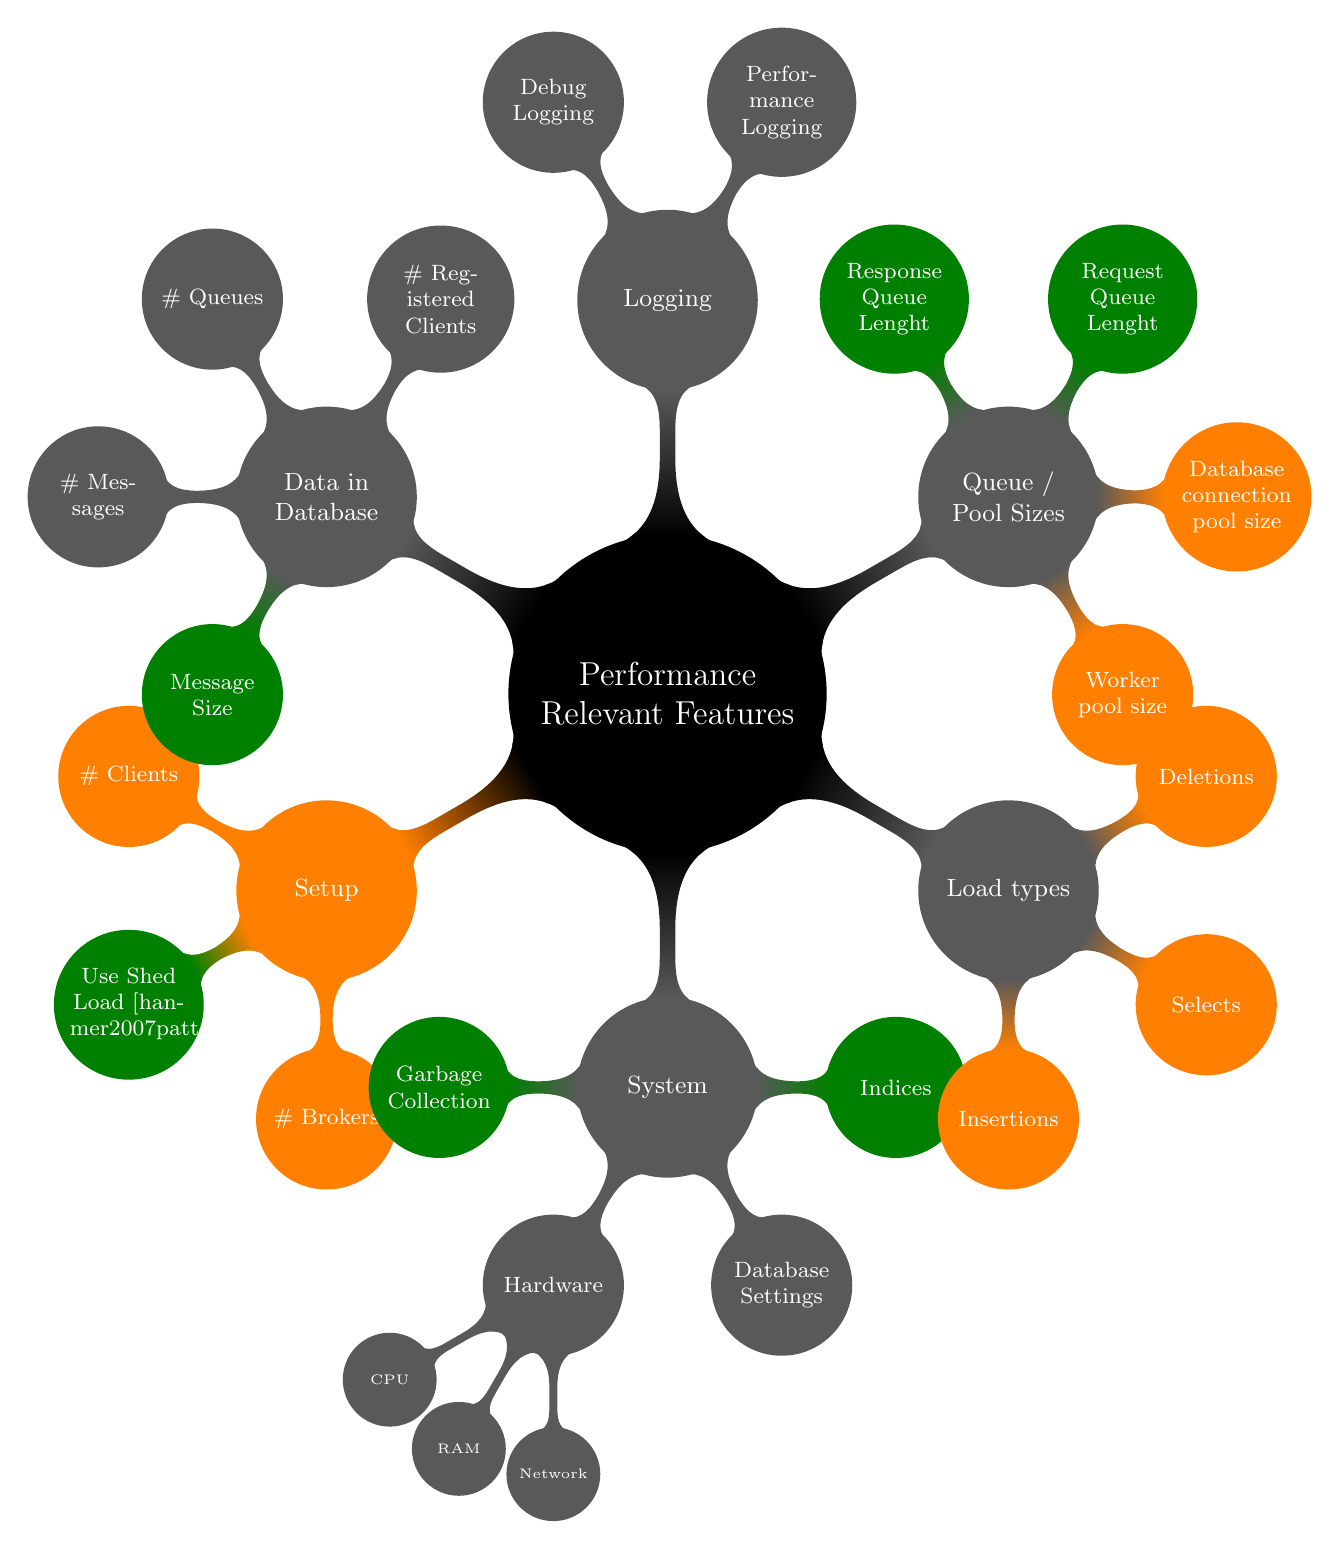
\begin{tikzpicture}[grow cyclic, align=flush center]
  \path[mindmap,concept color=black,text=white]
    node[concept] {Performance Relevant Features}
    %[clockwise from=0]
    child[concept color=orange] {
      node[concept] {Setup}
      child {
      	node[concept] {\# Clients} 
      }
      child[concept color=green!50!black] {
      	node[concept] {Use Shed Load [hanmer2007patterns]} 
      }
      child {
      	node[concept] {\# Brokers} 
      }
    }
    child[concept color=white!35!black] {
      node[concept] {System}
      child[concept color=green!50!black] { 
        node[concept] {Garbage Collection}
      }
      child { 
        node[concept] {Hardware}
        child { node[concept] {CPU} }
        child { node[concept] {RAM} }
        child { node[concept] {Network} }
      }
      child { 
        node[concept] {Database Settings}
      }
      child[concept color=green!50!black] { node[concept] {Indices}}
    }
    child[concept color=white!35!black] {
      node[concept] {Load types}
      child[concept color=orange] { 
      	node[concept] {Insertions} 
      }
      child[concept color=orange] {
      	node[concept] {Selects} 
      }
      child[concept color=orange] {
      	node[concept] {Deletions} 
      }
    }
    child[concept color=white!35!black] { 
      node[concept] {Queue / Pool Sizes}
      child[concept color=orange] { 
      	node[concept] {Worker pool size} 
      }
      child[concept color=orange] {
      	node[concept] {Database connection pool size} 
      }
      child[concept color=green!50!black] {
      	node[concept] {Request Queue Lenght} 
      }
      child[concept color=green!50!black] {
      	node[concept] {Response Queue Lenght} 
      }
    }
    child[concept color=white!35!black] { 
      node[concept] {Logging} 
      child { 
      	node[concept] {Perfor-mance Logging} 
      }
      child {
      	node[concept] {Debug Logging} 
      }
    }
    child[concept color=white!35!black] {
      node[concept] {Data in Database}
      child { 
      	node[concept] {\# Registered Clients} 
      }
      child {
      	node[concept] {\# Queues}
      }
      child {
      	node[concept] {\# Messages} 
      }
      child[concept color=green!50!black] {
      	node[concept] {Message Size} 
      }
    };
\end{tikzpicture}
\caption{Performance relevant features mind map} \label{fig:features_mindmap}
\end{figure}
%\end{landscape}

\subsection{Primary features}

According to figure~\ref{fig:features_mindmap}, the primary features are as follows:

\begin{enumerate}
  \item \textbf{\# Clients} The amount of clients interacting with the system.
  \item \textbf{\# Brokers} The amount of brokers interacting with the system.
  \item \textbf{Database connection pool size} The amount of database connections per broker to the database.
  \item \textbf{Worker pool size} The amount of workers per broker.
  \item \textbf{Insertions} When many insertions occur (send a message).
  \item \textbf{Deletions} When many deletions occur (read a message and remove it from the queue).
  \item \textbf{Deletions} When many deletions occur (read a message, but don't remove it from the queue).
\end{enumerate}


\subsection{Secondary features}

According to figure~\ref{fig:features_mindmap}, the secondary features are as follows:

\begin{enumerate}
  \item \textbf{Message Size} The average size of the messages payloads.
  \item \textbf{Use Shed Load} If the fault tolerance pattern Shed Load [hanmer2007pattern] is used or not.
  \item \textbf{Garbage Collection} The time it takes for the garbage collection.
\end{enumerate}


%% %%%%%%%%%%%%%%%%%%%%%%%%%%%%%%%%%%%%%%%%%%%%%%%%%%%%%%%%%%%%%%%%%%%%%%%%%
\section{How We Measured Our System}



\subsection{Hypothesis}

\section{References}

% TODO

http://dl.acm.org/citation.cfm?id=SERIES12798.1557393

@book{hanmer2007patterns,
  title={Patterns for fault tolerant software},
  author={Hanmer, Robert},
  year={2007},
  isbn = {0470319798, 9780470319796},
  publisher={Wiley Publishing}
}

%\bibliography{mybib}

%% %%%%%%%%%%%%%%%%%%%%%%%%%%%%%%%%%%%%%%%%%%%%%%%%%%%%%%%%%%%%%%%%%%%%%%%%%
\section{Notes - to delete}

\subsection{What should be included in this report }

\subsubsection{System Code}
\begin{itemize}
\item Code
\item Scripts for experiment
\end{itemize}

\subsubsection{Experimental data}
\begin{itemize}
\item Basic tests ans simple traces
\item Long running traces, Raw data and graphs for all experiments
\end{itemize}

\subsubsection{Written report}
\begin{itemize}
\item Architectural  diagrams
\item Interface description
\item explanation of the system design
\item Description of all experiments
\item statistical treatment of data
\item commentary analysis
\end{itemize}


\end{document}
